% Copyright © 2017-2018 Martin Ueding <dev@martin-ueding.de>
% Licensed under CC-BY 4.0

\documentclass{scrartcl}

\pagestyle{empty}

\usepackage{tikz}

\usetikzlibrary{arrows.meta}

\begin{document}

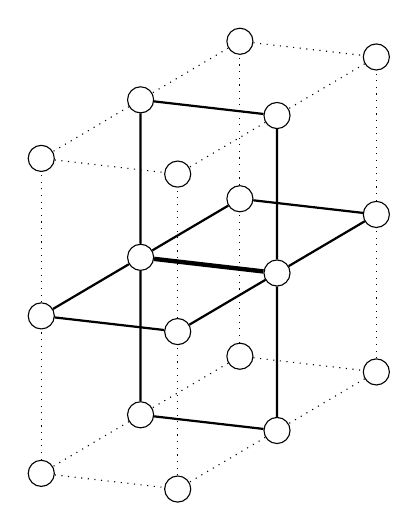
\begin{tikzpicture}[
        rotate around y=-15,
        %rotate around z=7,
        scale=2,
        link-main/.style={
            ultra thick,
        },
        link-staple/.style={
            thick,
        },
        link-needed/.style={
            dashed,
        },
        link-grid/.style={
            dotted,
        },
        point/.style={
            draw,
            circle,
        },
    ]

    % Lattice points.
    \foreach \x in {0, 1}
    \foreach \y in {0, 1, 2}
    \foreach \z in {0, 1, 2}
    \node[point] (n\x\y\z) at (\x, \y, \z) {};

    % Basic background grid.
    \foreach \a/\b in {0/1}
    \foreach \y in {0, 1, 2}
    \foreach \z in {0, 1, 2}
    \draw[link-grid] (n\a\y\z) -- (n\b\y\z);

    \foreach \x in {0, 1}
    \foreach \a/\b in {0/1, 1/2}
    \foreach \z in {0, 1, 2}
    \draw[link-grid] (n\x\a\z) -- (n\x\b\z);

    \foreach \x in {0, 1}
    \foreach \y in {0, 1, 2}
    \foreach \a/\b in {0/1, 1/2}
    \draw[link-grid] (n\x\y\a) -- (n\x\y\b);

    % Main link.
    \draw[link-main] (n011) -- (n111);

    % Staples.
    \draw[link-staple] (n011) -- (n021) -- (n121) -- (n111);
    \draw[link-staple] (n011) -- (n012) -- (n112) -- (n111);
    \draw[link-staple] (n011) -- (n010) -- (n110) -- (n111);
    \draw[link-staple] (n011) -- (n001) -- (n101) -- (n111);
\end{tikzpicture}

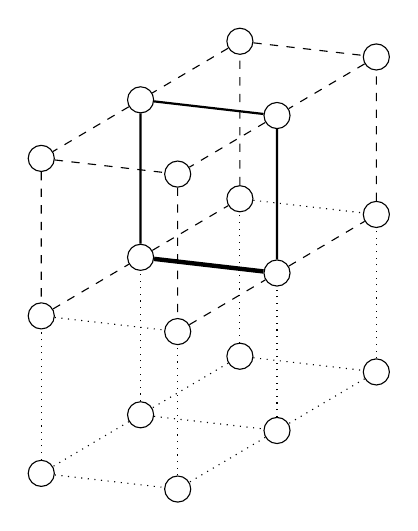
\begin{tikzpicture}[
        rotate around y=-15,
        %rotate around z=7,
        scale=2,
        link-main/.style={
            ultra thick,
        },
        link-staple/.style={
            thick,
        },
        link-needed/.style={
            dashed,
        },
        link-grid/.style={
            dotted,
        },
        point/.style={
            draw,
            circle,
        },
    ]

    % Lattice points.
    \foreach \x in {0, 1}
    \foreach \y in {0, 1, 2}
    \foreach \z in {0, 1, 2}
    \node[point] (n\x\y\z) at (\x, \y, \z) {};

    % Basic background grid.
    \foreach \a/\b in {0/1}
    \foreach \y in {0, 1}
    \foreach \z in {0, 1, 2}
    \draw[link-grid] (n\a\y\z) -- (n\b\y\z);

    \foreach \x in {0, 1}
    \foreach \a/\b in {0/1}
    \foreach \z in {0, 1, 2}
    \draw[link-grid] (n\x\a\z) -- (n\x\b\z);

    \foreach \x in {0, 1}
    \foreach \y in {0}
    \foreach \a/\b in {0/1, 1/2}
    \draw[link-grid] (n\x\y\a) -- (n\x\y\b);

    % Main link.
    \draw[link-main] (n011) -- (n111);

    % Staples.
    \draw[link-staple] (n011) -- (n021) -- (n121) -- (n111);

    % Links that are needed for the computation of the staple.
    \draw[link-needed] (n110) -- (n120) -- (n121) -- (n122) -- (n112) -- (n111) -- (n110);
    \draw[link-needed] (n010) -- (n020) -- (n021) -- (n022) -- (n012) -- (n011) -- (n010);
    \draw[link-needed] (n020) -- (n120);
    \draw[link-needed] (n022) -- (n122);
\end{tikzpicture}
    
\end{document}
